%!TEX root=Thesis.tex
\chapter{Evaluation}
\label{cha:evaluation}

Several experiments have been run in order to assess how well the implementation accomplishes the clause learning and clausal optimization tasks.
Moreover, the influence of different factors internal and external to the algorithm is evaluated.
The clause learning and clausal optimization workflows will be examined separately, in that order.

\section{Learning}

This section attempts to evaluate how well the clause learning system accomplishes the first goal of this thesis.
There are different aspects to be considered.
Firstly, the accuracy of the learned clauses will be examined, as well as the influence of several parameters on the accuracy.
This gives a measure of how well a learned theory approximates the underlying model.
Secondly, it will be evaluated how efficiently this task is accomplished.
Since clausal discovery can take a long time to find a theory on larger examples, it will be important to understand the influence of several factors on the running speed.
In the last part, the differences between learned clauses and constraints given by a user will be examined.

\subsection{Setup}
There are two key problems that are used to evaluate different questions.
Their standard setup will be described in this section.
Different experiments can vary on the specific examples and parameters that are used and it will be mentioned when this is the case.

\paragraph{Map coloring}
The map coloring problem has already been used as a running example in the previous section.
It also serves as a good, albeit small, example for clause learning in practice.
The standard setting uses two examples, each with three countries.
The first example (figure~\ref{fig:setup_mapcolor_benelux}) features two colors, while the second example (figure~\ref{fig:setup_mapcolor_benede}) needs three colors as all countries are connected.

\begin{figure}
\centering
\begin{minipage}{.5\textwidth}
  \centering
  \includegraphics[height=3.5cm]{MapColoringBenelux.pdf}
  \caption{Map coloring example 1}
  \label{fig:setup_mapcolor_benelux}
\end{minipage}%
\begin{minipage}{.5\textwidth}
  \centering
  \includegraphics[height=3.5cm]{MapColoringBenede.pdf}
  \caption{Map coloring example 2}
  \label{fig:setup_mapcolor_benede}
\end{minipage}
\end{figure}

Map coloring uses types $\mathit{Country}$ and $\mathit{Color}$.
It uses two predicates $\mathit{color/2}$ and $\mathit{neighbor/2}$, the neighbor predicate is symmetric.
Unless mentioned otherwise, the standard parameters for map coloring are $3$ variables and~$3$ terms per clause.

\paragraph{Sudoku}
Sudoku is a slightly more difficult problem.
An $n \times n$ sudoku contains $n$ rows, $n$ columns and $n$ blocks, each of which contains the numbers $1$ to $n$ exactly once.
Every cell is represented by an object of type $\mathit{Cell}$.
The other types describe attributes of cells: $\mathit{Row}$, $\mathit{Colum}$, $\mathit{Block}$ and a numeric type $\mathit{Value}$.
Each of those attributes is related to a cell through the predicates $\mathit{row/2}$, $\mathit{col/2}$, $\mathit{block/2}$ and $\mathit{value/2}$ respectively.
In the standard setting one $4 \times 4$ example (figure~\ref{fig:setup_sudoku}) is provided.

\begin{figure}[!htp]
	\centering
	\begin{tabular}{|cc|cc|}
		\hline
		1 & 3 & 2 & 4 \\
		4 & 2 & 3 & 1 \\ \hline
		2 & 1 & 4 & 3 \\
		3 & 4 & 1 & 2 \\ \hline
	\end{tabular}
	\label{fig:setup_sudoku}
	\caption{$4 \times 4$ sudoku example}
\end{figure}

Clause learning on the sudoku is usually done with $4$ variables and~$4$ terms per clause.
In the example, the row, column, block and value are explicitly given for each cell.
The use of specific, disjoint types instead of one common (numeric) type for rows, columns and blocks makes the clause learning process more efficient.
It prevents the use of the same variable for, for example, a row and a column.

\paragraph{Elevator}

\paragraph{Co-housing}
The co-housing problem is a somewhat more complex problem.
Two friends (persons) are looking at different situations (areas) to live and work in.
\\\\
\begin{minipage}{0.5\textwidth}
	\begin{verbatim*}
		type Area
		type Person
		type Cost > nat

		calc cheap(Cost)
	\end{verbatim*}
\end{minipage}
\begin{minipage}{0.5\textwidth}
	\begin{verbatim*}
		pred live(Person, Area)
		pred work(Person, Area)
		pred car(Person)

		pred cost(Area, Cost)
	\end{verbatim*}
\end{minipage}

Background knowledge is used to calculate what is considered as cheap. It also limits the amount of people to $2$ and expresses that every area has only one cost. There are $5$~examples that each adhere to $4$~constraints:

\begin{enumerate}
	\item If the two persons do not live in the same area, they work in the same area.
	\item If a person does not work and live in the same area, that person needs a car.
	\item A person who lives in a cheap area has a car
	\item If the two persons live together, they live in an expensive area.
\end{enumerate}

\subsection{Accuracy}

\# Q : Does the learned theory express the model
% - P Observation (Additional [-> IDP?] | Essential | Damaging)
% - N Test examples

\# Q : Influence parameters
% - C Influence number terms / variables
% - N Dependent of size / number of examples
% - C Influence range restriction

\subsection{Speed}

Unless explicitly stated, all problems are run $8$ consecutive times in order to eliminate external influences.
The experiments are run on the same machine\footnote{Mac OSX, 2.3 GHz Intel Core i7 with 4 cores and hyper threading, 16GB RAM}.

\begin{question}
	How fast is the clause learning system?
\end{question}

\begin{experiment}
	In order to gain an overview over the running times and provide a benchmark for tests on various influences, the standard examples are each run using the standard clause learning process.
	
	\begin{table}[!htp]
		\begin{tabularx}{\textwidth}{XXX}
			\textbf{Name}	& \textbf{Mean (s)}	& \textbf{StdDev (s)} \\
			\toprule
			Map coloring 	& 1.581				& 0.117 \\
			Sudoku 			& 4.787				& 0.062 \\
			Elevator 		& 3.182 			& 0.073 \\
			Co-housing 		& 25.903			& 0.446
		\end{tabularx}
		\label{tbl:exp_speed_standard}
		\caption{Running times for standard examples}
	\end{table}

\end{experiment}

% - N Compared with others?

\paragraph{Discussion}
"Discuss"

\begin{question}
	What is the influence of the various parameters and input data?
\end{question}

% - C Influence number terms / variables
% - N Influence number examples
% - N Influence arity

\begin{question}
	How do the syntactic restrictions influence the running time?
\end{question}

\begin{experiment}[\textsc{Range restriction}]
	The clause learning algorithm normally only explores range restricted clauses.
	While this measure positively influences the efficiency of the algorithm, it trades off expressiveness.
	In this experiment the standard problems are run, while allowing lifting the constraint that clauses must be range restricted.

	\begin{table}[!htp]
		\begin{tabularx}{\textwidth}{XXX}
			\textbf{Name}	& \textbf{Mean (s)}	& \textbf{StdDev (s)} \\
			\toprule
			Map coloring 	& 4.629				& 0.199 \\
			Sudoku 			& 16.118			& 0.154 \\
			Elevator 		& 40.453 			& 0.319 \\
			Co-housing 		& 207.768			& 0.330
		\end{tabularx}
		\label{tbl:exp_speed_no_range}
		\caption{Running times for standard examples without range restriction}
	\end{table}

\end{experiment}

\begin{experiment}[\textsc{Connected clauses}]
	"Write"

	\begin{table}[!htp]
		\begin{tabularx}{\textwidth}{XXX}
			\textbf{Name}	& \textbf{Mean (s)}	& \textbf{StdDev (s)} \\
			\toprule
			Map coloring 	& 1.589				& 0.110 \\
			Sudoku 			& 7.068				& 0.150 \\
			Elevator 		& 6.157 			& 0.114 \\
			Co-housing 		& 103.633			& 0.131
		\end{tabularx}
		\label{tbl:exp_speed_no_connect}
		\caption{Running times for standard examples without connectivity}
	\end{table}

\end{experiment}

\paragraph{Discussion}
"Discuss"

\begin{question}
	What is the influence of the efficiency measures on the running time?
\end{question}

There are mainly two measures incorporated in the clause learning algorithm that aim to reduce the running time.
Contrary to syntactic restrictions these do, in principle, not affect the outcome of the algorithm.

\begin{experiment}[\textsc{Symmetric predicates}]
	The first design choice evaluated is the option to provide symmetric predicates.
	The map coloring example contains a symmetric predicate $\mathit{neighbor}$.
	By replacing this symmetric predicate with a standard predicate, the influence on the running time can be measured.

	\begin{table}[!htp]
		\begin{tabularx}{\textwidth}{XXX}
			\textbf{Name}	& \textbf{Mean (s)}	& \textbf{StdDev (s)} \\
			\toprule
			Standard & 1.581 & 0.117 \\
			Non-symmetric & 2.541 & 0.128 \\
		\end{tabularx}
		\label{tbl:exp_speed_symm}
		\caption{Running times symmetric vs. non-symmetric map coloring}
	\end{table}

	By running the non-symmetric version $8$ times, it can be compared to the standard map coloring problem.
	In the non-symmetric version an additional constraint is learned to express the symmetry of the neighbor relation: \cen{$\mathit{neighbor}(c_2, c_1) \leftarrow \mathit{neighbor}(c_1, c_2)$.}
\end{experiment}

\begin{experiment}[\textsc{Subset test}]
	As mentioned in chapter~\ref{cha:meth}, a subset test is used to forestall some entailment tests.
	In this experiment, the running times without subset test is measured to evaluate the effect of this test.
	To this end, the standard problems are run without the subset test.

	\begin{table}[!htp]
		\begin{tabularx}{\textwidth}{XXX}
			\textbf{Name}	& \textbf{Mean (s)}	& \textbf{StdDev (s)} \\
			\toprule
			Map coloring 	& 1.558				& 0.117 \\
			Sudoku 			& 5.239				& 0.140 \\
			Elevator 		& 3.678 			& 0.094 \\
			Co-housing 		& 30.145			& 0.159
		\end{tabularx}
		\label{tbl:exp_speed_no_subset}
		\caption{Running times for standard examples without subset test}
	\end{table}
\end{experiment}

\begin{experiment}[\textsc{Representative test}]
	The same constraint can often be represented by multiple clauses.
	In order to avoid generating different clauses but equivalent, the refinement operator defines an order of clauses.
	If a clause cannot be rewritten as a different clause that occurs earlier in that order, the clause is called representative.
	This measure leads to a reduction of generated clauses.
	In this experiment the standard problems are run without this test.

	\begin{table}[!htp]
		\begin{tabularx}{\textwidth}{XXX}
			\textbf{Name}	& \textbf{Mean (s)}	& \textbf{StdDev (s)} \\
			\toprule
			Map coloring 	& 2.389				& 0.130 \\
			Sudoku 			& 8.995				& 0.125 \\
			Elevator 		& 3.559 			& 0.076 \\
			Co-housing 		& 55.402			& 0.298
		\end{tabularx}
		\label{tbl:exp_speed_no_representative}
		\caption{Running times for standard examples without representative test}
	\end{table}

\end{experiment}

\paragraph{Discussion}
"Discuss"

\subsection{Compared to human}

\begin{question}
	What is the relation between machine learned and user provided clauses?
\end{question}

% - P Damaging vs. errors
% - P No redundant clauses
% - P More expressiveness

\paragraph{Discussion}
"Discuss"

\section{Optimization}
This section examines how well the second goal of the thesis, the learning of optimization criteria, has been accomplished.
Contrary to the previous section, the evaluation will focus only on the accuracy with which the learned soft constraints are able to approximate an underlying model.
Different factors will be explored that influence the results of the clausal optimization system.

\subsection{Setup}

\paragraph{Housing}
The primary example for clausal optimization revolves around housing.
There are three areas ($A_1$, $A_2$ and $A_3$) which have certain characteristics such as whether the area has a low crime rate and is cheap to live in.
In this example the user is trying to decide 1) where to live, 2) where to work and 3) which school to select.
Any area can be chosen for living and all areas have a school.
The areas to work in are restricted by the job offers that have been received.

\begin{table}[!htp]
	\begin{tabularx}{\textwidth}{l|r||*3{>{\centering\arraybackslash}X}}
	    & \textbf{Category} & \textbf{Area 1} & \textbf{Area 2} & \textbf{Area 3} \\
	    \midrule
	    \textbf{Properties} & Low crime & x & x & \\
	    & Cheap & x & & x \\
	    \midrule
	    \textbf{Possible} & House & x & x & x \\
	    \textbf{locations} & Job offer & x & x & \\
	    & School & x & x & x 
	\end{tabularx}
	\label{tbl:setup_housing}
	\caption{Characteristics and restrictions}
\end{table}

The different possible choices form $18$ distinct examples.
Using variables $x, y$ and~$z$ to denote the selected living, work and school areas, respectively, a template example can be formulated as:

\begin{figure}[!htp]
	\begin{minipage}{0.5\textwidth}
		\begin{verbatim*}
			const Area A1 A2
			const Area A3 A4

			low_crime(A1)
			low_crime(A2)
			low_crime(A4)
		\end{verbatim*}
	\end{minipage}
	\begin{minipage}{0.5\textwidth}
		\begin{verbatim*}
			cheap(A1)
			cheap(A3)

			live_in(x)
			work_in(z)
			school_in(y)
		\end{verbatim*}
	\end{minipage}
	\label{fig:setup_housing_example_template}
	\caption{Housing example template}
\end{figure}

In order to emulate real user preferences, a model is used used to generate pair wise rankings over the examples.
The standard model consists of $4$ weighted constraints:
\begin{shiftedflalign*}
	& \text{ }0.50 : \mathit{low\_crime}(a) \leftarrow \mathit{live\_in}(a) & \\
	& \text{ }0.25 : \mathit{school\_in}(a) \leftarrow \mathit{work\_in}(a) & \\
	& \text{ }1.00 : \mathit{low\_crime}(a) \leftarrow \mathit{school\_in}(a) & \\
	& \text{-}1.00 : \mathit{false} \leftarrow \mathit{live\_in}(a) \land \mathit{cheap}(a) &
\end{shiftedflalign*}

\subsection{Accuracy}

Generally, the experiments in this section follow one of two approaches.
\begin{description}
	\item[Approach 1] The available examples are split into two parts: the training and the test set.
	\item[Approach 2] All examples are used both as training and test set.
\end{description}
Both approaches then follow the same process, which is visualized in figure~\ref{fig:co_test_setup}.

First, all pairwise rankings over the examples in the training set are generated using the model constraints and a fraction of these are selected.
A fraction of these remaining rankings are then inverted to simulate noise.
The clausal optimization process is used to generate soft constraints which in turn are used generate pairwise ratings over the test set.
These pairwise rankings are compared to the pairwise rankings generated over the test set by the model constraints.
By counting the number of rankings that disagree and dividing this by the total number of rankings, one obtains the Kendall tau distance $\mathit{KD}$.
The score is calculated as $1 - \mathit{KD}$.

\begin{figure}

	\caption{Clausal optimization testing setup}
	\centering
		\includegraphics[width=1\textwidth]{COSetup.pdf}
	\label{fig:co_test_setup}

\end{figure}


\begin{question}
	How accurately can soft constraints learned through clausal optimization approximate the underlying model?
\end{question}


% - A On same examples
% - A Ranging size examples / preferences

\paragraph{Discussion}
"Discuss"

\begin{question}
	What is the influence of noise on the learned optimization criteria?
\end{question}

\begin{experiment}[\textsc{Influence of noise}]
	In order to answer this question, this experiment primarily measures the influence of the amount of inverted rankings in the second approach.
	The housing example was run for varying fractions of rankings and varying fractions of noise.
	Figure~\ref{fig:nosplit_noise_noise} shows the effect of increasing noise on the score for several fractions of rankings.
	On figure~\ref{fig:nosplit_noise_rankings} the effect of increasing the amount of rankings can be seen, when the noise level is fixed.

	\begin{figure}

		\caption{Score for increasing noise}
		\centering
			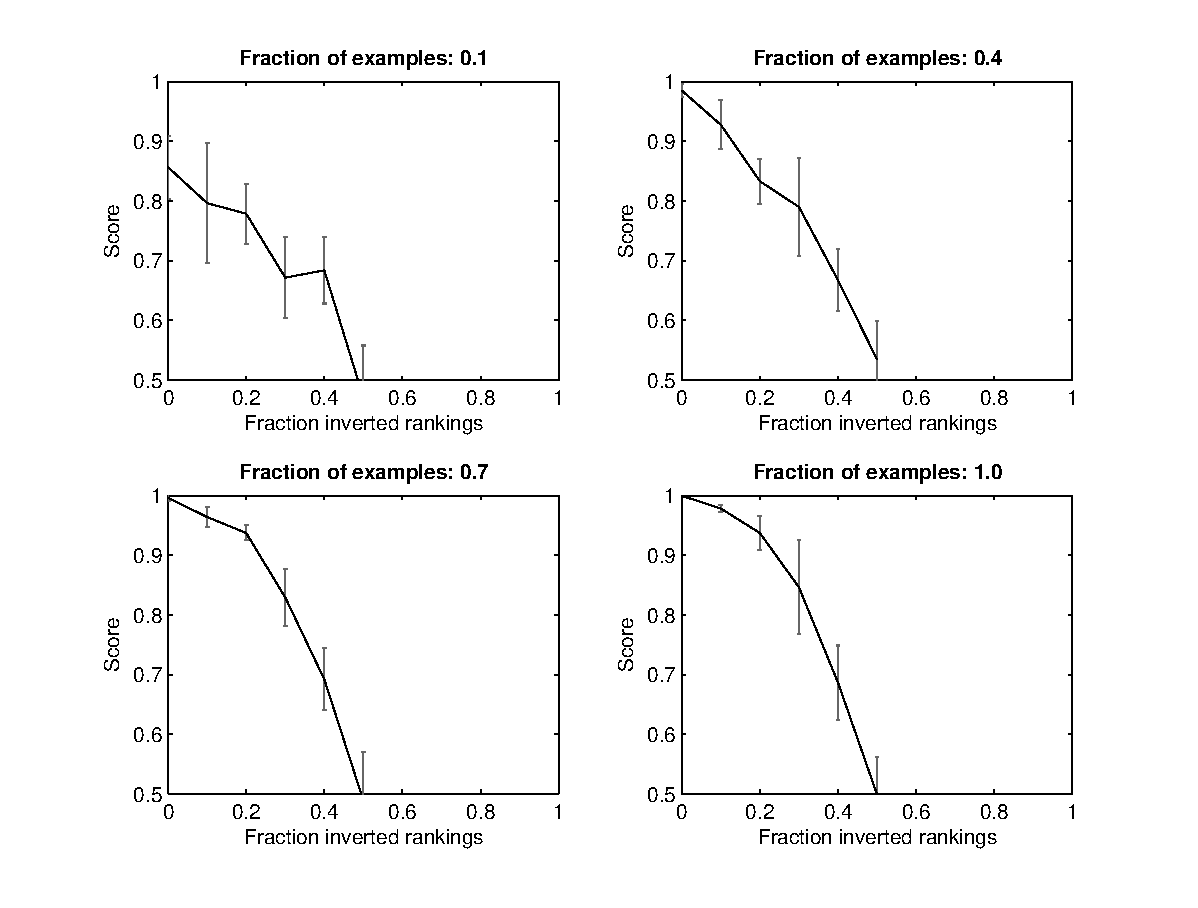
\includegraphics[width=.8\textwidth]{nosplit_noise_noise}
		\label{fig:nosplit_noise_noise}

	\end{figure}

	\begin{figure}

		\caption{Effect of increasing fraction of rankings}
		\centering
			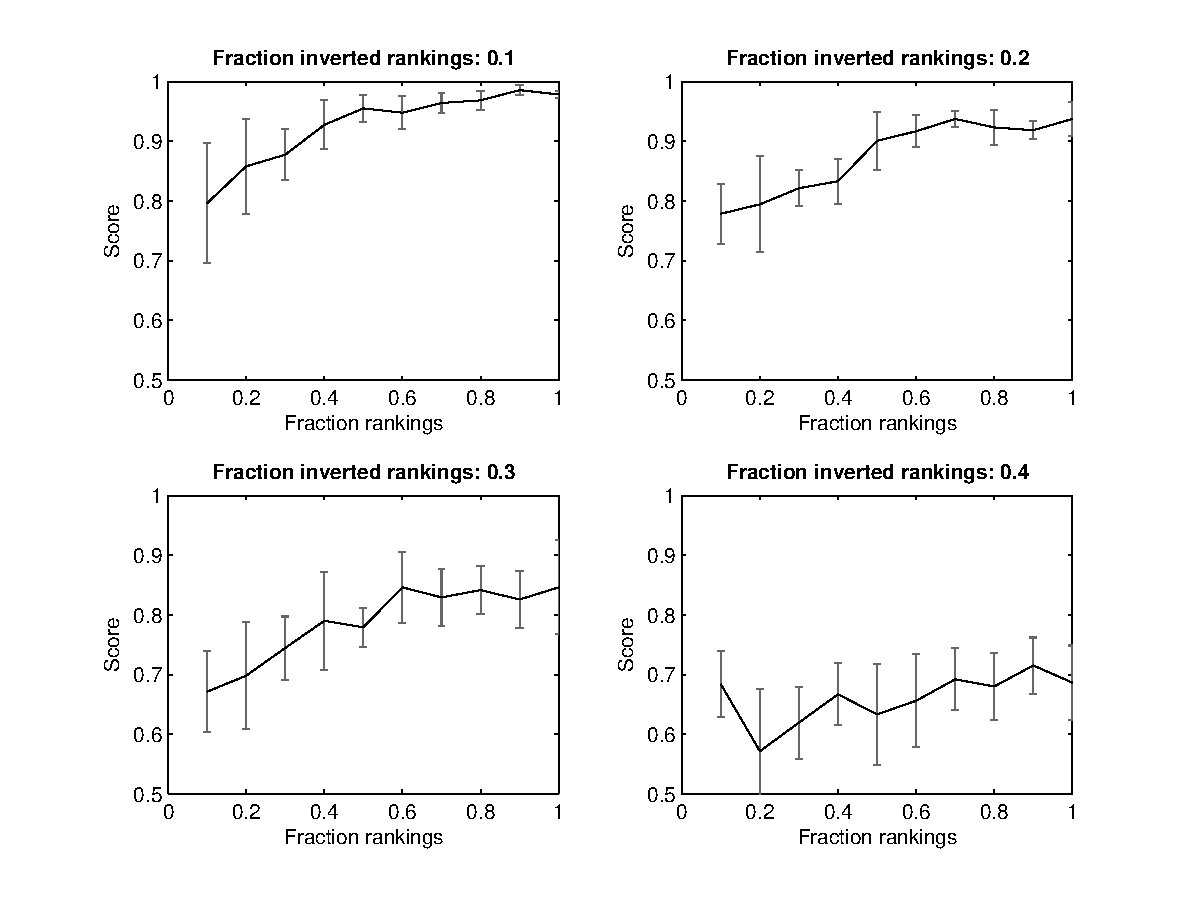
\includegraphics[width=.8\textwidth]{nosplit_noise_rankings}
		\label{fig:nosplit_noise_rankings}

	\end{figure}

\end{experiment}

\begin{experiment}[\textsc{Noise in approach 1}]
	
	The influence of noise is similar for approach~1.
	Figure~\ref{fig:hard_constraints} shows how the standard implementation (with hard constraints for pruning) performs for increasing noise levels.

\end{experiment}

% - C Formulation of rankings (a > b > c vs. a > b, b > c)

\paragraph{Discussion}
"Discuss"


\begin{question}
	What is the effect of internal parameters or influences?
\end{question}

The experiments for this question explore the influence of several factors.
Unless mentioned otherwise, the experiments will use the following setup as baseline:
Approach~1, where the fraction of examples in the training set is chosen as $0.4$ and the fraction of rankings is also set to $0.4$.

% - P other kernel

\begin{experiment}
	
	Clausal optimization uses a cost factor which represents the cost of disagreeing with a provided ranking in favor of a simpler model (see section~\ref{sec:clausal_opt_approach}).
	This parameter can help avoid overfitting.
	The standard setting in the clausal optimization is $0.2$.
	In this experiment the influence of the cost factor has been measured for different noise levels.
	Figure~\ref{fig:c_factors} shows the influence of the cost factor on the score for fixed noise levels.

	\begin{figure}

		\caption{Influence of cost factor}
		\centering
			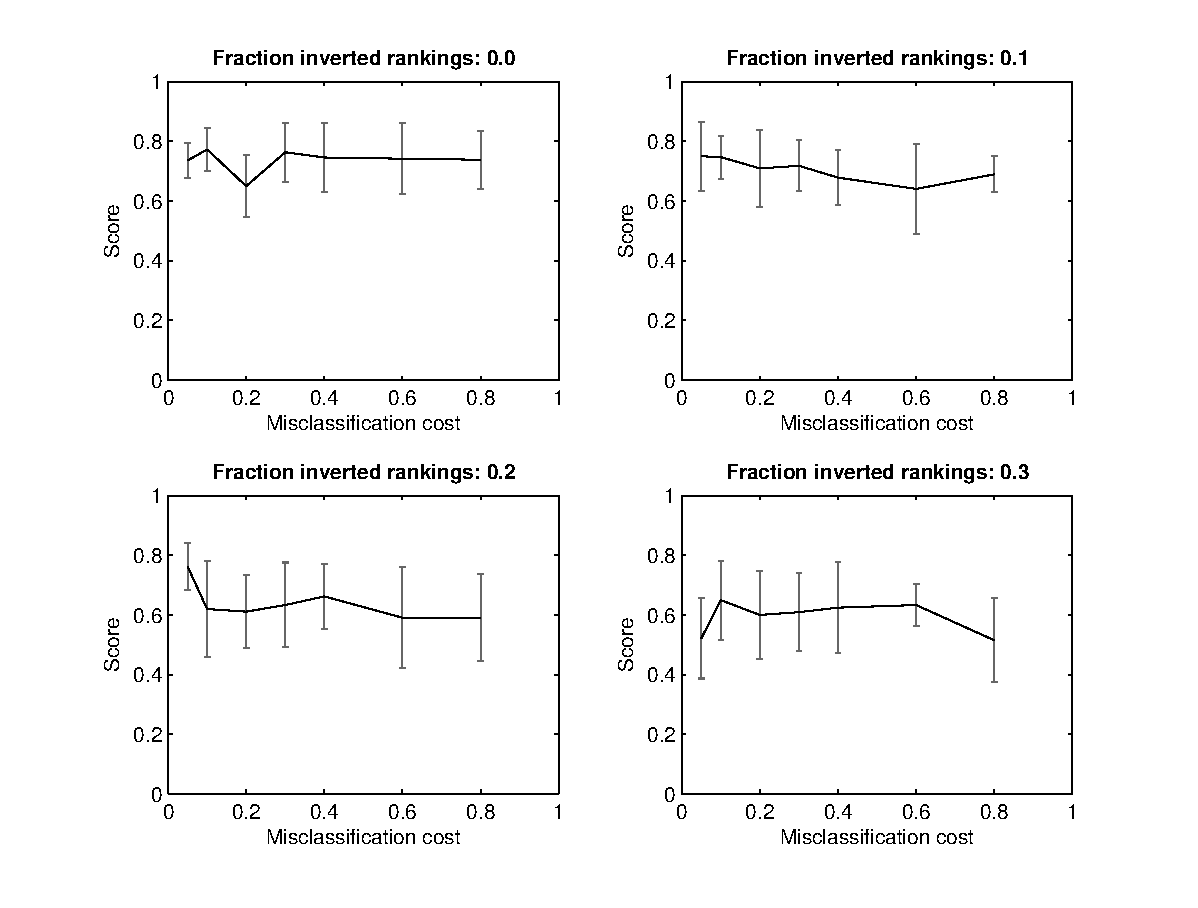
\includegraphics[width=.8\textwidth]{c_factors}
		\label{fig:c_factors}

	\end{figure}

\end{experiment}

\begin{experiment}
	
	In the clause learning implementation the choice was made to allow hard constraints to prune soft constraints (see section~\ref{sec:clausal_discovery_approach}).
	This simplfies the model as fewer clauses are learned at the expense of pruning some clauses with discriminative power if the hard constraints just coincidently cover all the given examples.
	This experiment compares the standard implementation with an alternative implementation that does not allow hard constraints to prune for increasing noise levels.
	The results can be seen in figure~\ref{fig:hard_constraints}.

	\begin{figure}

		\caption{Pruning with and without hard constraint}
		\centering
			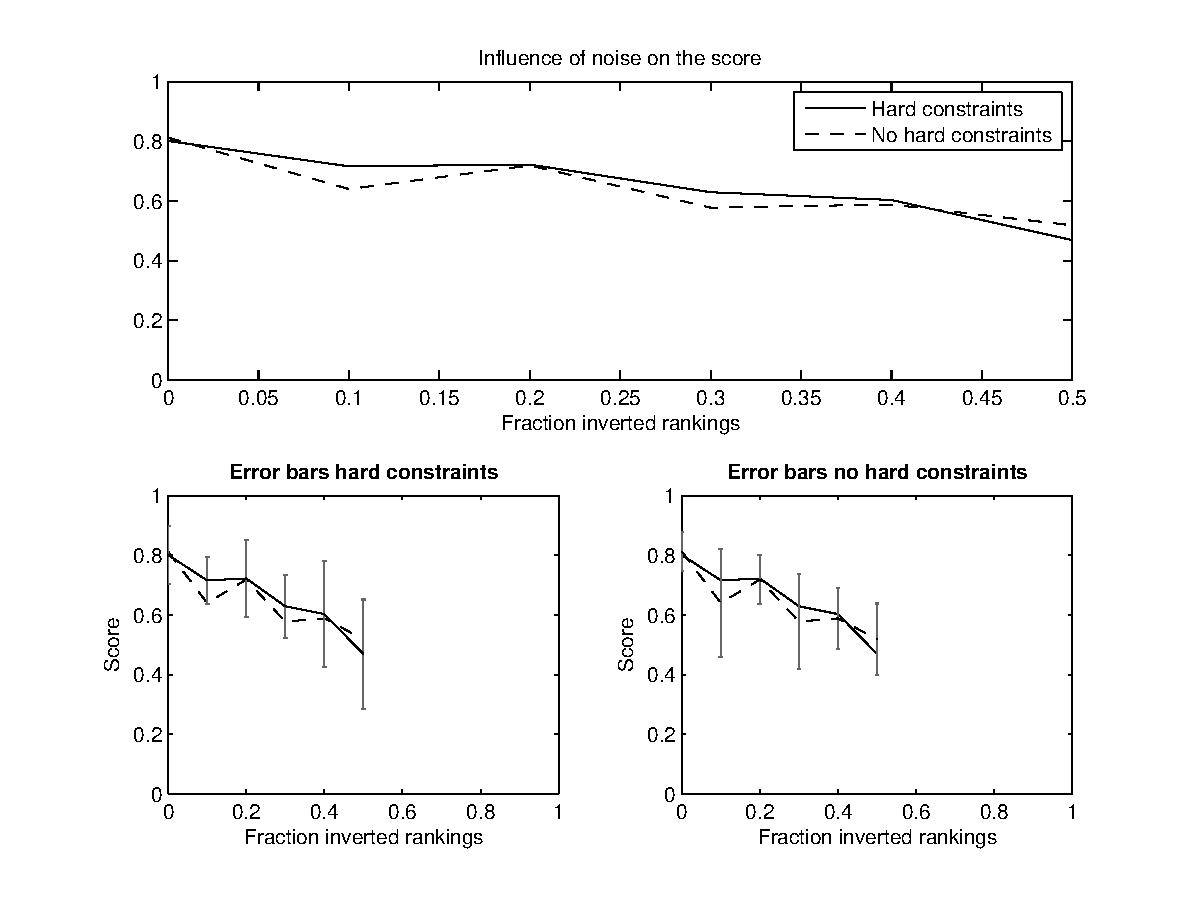
\includegraphics[width=.8\textwidth]{hard_constraints}
		\label{fig:hard_constraints}

	\end{figure}

\end{experiment}

\paragraph{Discussion}
"Discuss"

\# "Q : Expressivity"
% - A On same examples
% - N Different underlying models

